

\begin{frame}
  \frametitle{Progress chart}       
  	  \begin{textblock*}{12.5cm}(0.1cm,3cm) % {block width} (coords)
 \begin{figure}[ht!] % replace 't' with 'b' to force it to 
	\includegraphics[width=\textwidth]{./images/progress_chart_light.pdf} 
	\caption{Workflow for the simulations proposed in this work.}
\end{figure}
		\end{textblock*}
\end{frame}


\subsection{Stage 1: Basic on-line reprocessing demonstration}


\begin{frame}
\frametitle{Stage 1 goals (complete)}
	\begin{itemize}
		\itemsep1em
		\item Review and summarize state of the art
		\item Create \textbf{high-fidelity full-core model} of the \gls{MSBR} 
		in Serpent
		\item Simple SaltProc v0.1 demonstration and validation for 
		once-through \gls{MSR} reprocessing \textbf{(``black box'') with 
		fixed, ideal $\epsilon_e$}
		\item \textbf{Equilibrium fuel composition} search for the \gls{MSBR} 
		based on ideal removals
		\item Investigate \textbf{effect of \gls{FP} removal}
	\end{itemize}

\end{frame}

\begin{frame}
\frametitle{Stage 1 results: multiplication factor dynamics}

\begin{columns}
	\column{4.3cm}
	\begin{block}{\gls{MSBR} on-line reprocessing analysis}
		\fontsize{7}{9}\selectfont
		\begin{itemize}
			\item Full-core model of the \gls{MSBR} for 60 years of operation
			\item FP removal from the salt with fixed, ideal extraction 
			efficiencies 
			\item $^{233}$Pa ideal removal and feed of an equal mass of 
			$^{233}$U into the core
			\item Fresh fertile material feed to maintain the salt inventory
			\item Fine time resolution (3-day depletion steps)
		\end{itemize}
	\end{block}    	
	
	\column{8cm}
		\begin{figure}[ht!] 
		\centering
			\includegraphics[width=\textwidth]{../figures/keff_msbr.png}
			\caption{Effective multiplication factor dynamics for the 
			full-core \gls{MSBR} model (reproduced from  
			Rykhlevskii \emph{et al.} \cite{rykhlevskii_modeling_2019}).}
		\end{figure}
	
\end{columns}
\end{frame}


\begin{frame}
\frametitle{Stage 1 results: Effect of fission products removal}       

\begin{figure}[t] % replace 't' with 'b' to force it to 
	\centering
	\includegraphics[width=0.8\textwidth]{../figures/keff_rem_cases.png} 
	\caption{Calculated effective multiplication factor for the full-core 
		\gls{MSBR} model with removal of various fission product groups over 
		10 	years of operation (reproduced from Rykhlevskii \emph{et al.} 
		\cite{rykhlevskii_modeling_2019}).}
\end{figure}

\end{frame}



\subsection{Stage 2: Tool demonstration and validation for \gls{TAP}}

\begin{frame}
\frametitle{Stage 2 goals (in progress)}
\begin{enumerate}
	\itemsep1em
	\item Review and summarize the \gls{TAP} reactor and \textbf{fuel 
	reprocessing system design}
	\item Create \textbf{high-fidelity full-core model} of the \gls{TAP} core 
	in Serpent
	\item Develop multi-component fuel reprocessing system model with 
	\textbf{fixed, non-ideal removal efficiency}
	\item SaltProc demonstration for fixed removal 
	efficiency and static geometry
	\item Enable switching between multiple Serpent
geometries during 
	simulation to \textbf{maintain the \gls{TAP} core criticality}
	\item Perform 40-year depletion simulation using SaltProc and 
	\textbf{compare} obtained results with Betzler \emph{et al.} 
	\cite{betzler_assessment_2017}
\end{enumerate}

\end{frame}

\begin{frame}
\frametitle{\gls{TAP} concept high-fidelity Serpent model}
	  \begin{textblock*}{12.25cm}(0.25cm,1.8cm) % {block width} (coords)
\begin{figure}[htp!] % replace 't' with 'b' to 
	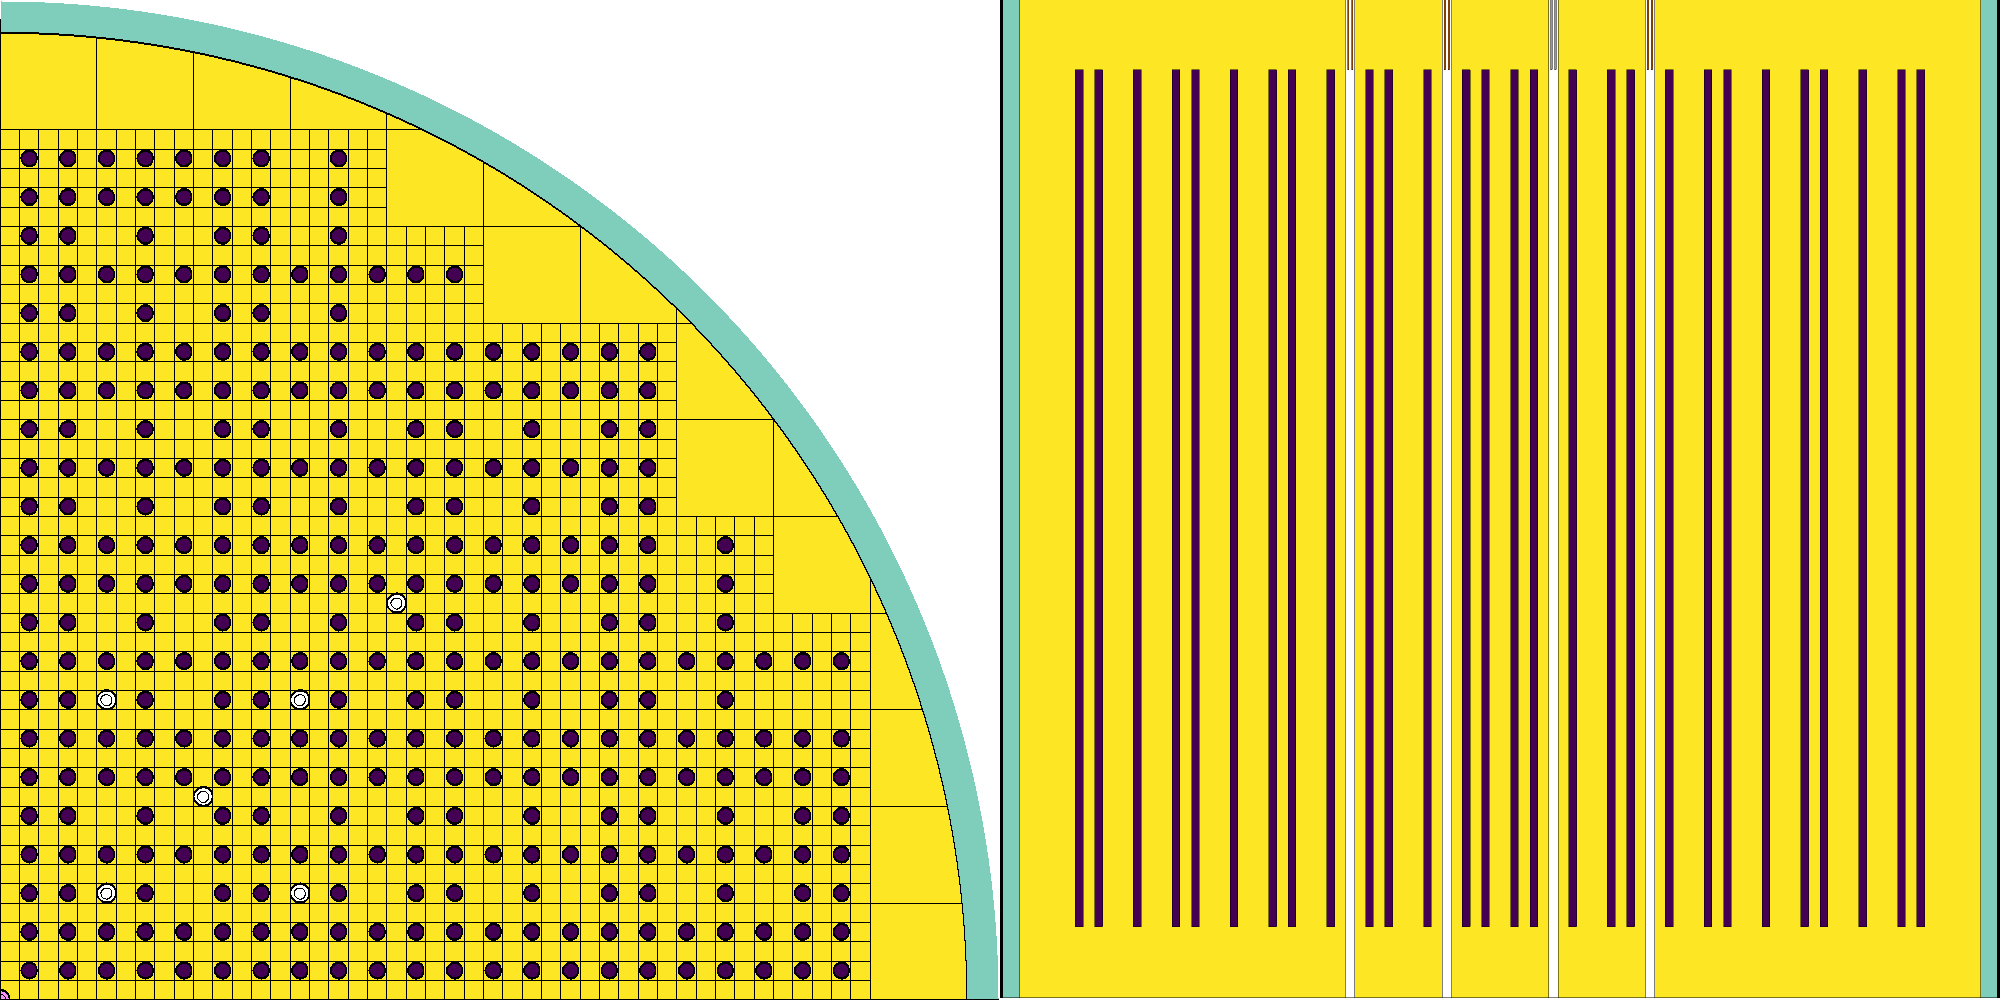
\includegraphics[width=\textwidth]{./images/tap_model.png}
	\caption{An $XY$ (left) and $XZ$ (right) section of the \gls{TAP} model. 
	The violet color represents zirconium hydride, and the yellow represents 
	fuel salt (reproduced from Rykhlevskii \& Huff 
	\cite{rykhlevskii_milestone_2019}).}
\end{figure}
	  \end{textblock*}
\end{frame}


\begin{frame}
\frametitle{Multi-component fuel reprocessing system model in SaltProc}       

\begin{columns}
		\column[t]{6cm}
		\begin{itemize}
			\item Fixed, non-ideal ($<100\%$) removal efficiencies
			\item Sparger and separator located in-line
			\item Static geometry with constant moderator-to-fuel ratio
			\item 5\% and 19.79\% low-enriched uranium feed
		\end{itemize}

	\column[t]{6.5cm}
	\begin{figure}[htp!] % replace 't' with 'b' to 
	\centering
			\vspace{-7mm}
		\begin{overprint}
	\onslide<1>\includegraphics[height=0.8\textheight]{../figures/demo_reprocessing_scheme.png}
	\onslide<2>\includegraphics[height=0.8\textheight]{../figures/demo_reprocessing_scheme_2.png}
		\end{overprint}
	\caption{\gls{TAP} reprocessing scheme flowchart used for demonstration of 
		SaltProc \cite{rykhlevskii_milestone_2019}.}
	\end{figure}
\end{columns}
\end{frame}


\begin{frame}
\frametitle{Depletion simulation results for TAP with various feeds}       
\begin{textblock*}{12.6cm}(0.1cm,2.2cm) % {block width} (coords)
	\begin{figure}[htp!] % replace 't' with 'b' to 
		\begin{minipage}[b]{0.48\textwidth}
			\includegraphics[width=\linewidth]{../figures/keff_3.png}
		\end{minipage}
			\hspace{-2mm}
		\begin{minipage}[b]{0.48\textwidth}
			\includegraphics[width=\linewidth]{../figures/keff_zoomed_2.png}
		\end{minipage}
		\caption{Effective multiplication factor dynamics for full-core
		\gls{TAP} model for different fueling scenarios over a 13-year reactor 
		operation (left) and for the time interval from 367 to 471 days after 
		startup (right). Confidence interval $\pm\sigma=28pcm$ is shaded.}
	\end{figure}
\end{textblock*}
\end{frame}


\begin{frame}
\frametitle{Fuel salt composition evolution during the TAP operation}
\begin{textblock*}{12.25cm}(0.25cm,1.8cm) % {block width} (coords)
	\begin{figure}[htp!] % replace 't' with 'b' to 
		\centering
				\vspace{-3mm}
		\includegraphics[width=0.72\textwidth]{../figures/u_pu_mass.png}
		\caption{Mass of major nuclides during 13 years of reactor operation 
		with 19.79\% \gls{LEU} feed.}
	\end{figure}
\end{textblock*}
\end{frame}

%\begin{frame}
%\frametitle{SaltProc demonstration for realistic on-line reprocessing system}
%\begin{block}{Finishing Stage 2}
%	\begin{enumerate}
%		\item Implement variable core geometry capability in SaltProc
%		\item Demonstrate a key feature of
%		the \gls{TAP} reactor - 
%		adjusting the moderator rod configuration - which is necessary 
%		achieve 60-years lifetime.
%		\item Perform 40-year depletion simulation using SaltProc 
%		and compare obtained results with Betzler \emph{et al.} 
%		\cite{betzler_assessment_2017}
%	\end{enumerate}
%\end{block}
%\end{frame}


\subsection{Stage 3\&4: Variable Xe removal and gas removal system bounding}


\begin{frame}
	\frametitle{Stage 3 (in progress): SaltProc demonstration with variable 
	$\epsilon_{Xe}$}
	\begin{columns}
	\column{7cm}
\begin{block}{Realistic fuel processing system model for the \gls{TAP}}
	\begin{enumerate}
		\itemsep1em
		\item Incorporate extraction efficiencies as a \textbf{function of 
		many physical system design	parameters} (e.g., helium bubble size)
		\item Perform life-time long depletion simulation with \textbf{dynamic 
		removal efficiency}
		\item Perform short-term (3 days) in \textbf{load-following regime}
		\item Conduct \textbf{parametric sweep of input parameters} in 
		$\epsilon_{Xe}$ 
		equation to determine the range of key parameters
	\end{enumerate}
\end{block}
	\column{4.5cm}
	\begin{figure}[bth!] % replace 't' with 'b' to 
		\centering
		\includegraphics[width=1.1\textwidth]{../figures/load_curve.png}
		\caption{Tentative load curve for short-term simulation.}
		\label{fig:load}
	\end{figure}
	\end{columns}
\end{frame}



\begin{frame}
\frametitle{Gas removal system bounding for the TAP}

\begin{block}{Stage 4: Prototype design for the xenon removal system}
	\begin{enumerate}
		\itemsep1em
		\item \textbf{Determine bounds for key design parameters} (sparger 
		volume, geometry, salt and helium flow rates) by analyzing parametric 
		sweep
		\item Calculate key design parameters to \textbf{minimize fuel salt 
		inventory} in the system
		\item Perform \textbf{nuclear criticality safety} analysis using MCNP6 
		\cite{werner_mcnp6._2018} to confirm that the selected sparger design 
		is safe
	\end{enumerate}
\end{block}
\end{frame}


\subsection{Stage 5: Safety parameters evolution}

\begin{frame}
\frametitle{\gls{TAP} Safety and Operational parameters analysis}
		\begin{block}{Stage 5: Safety parameters dynamics for 
		long- and short-term depletion}
	\begin{enumerate}
		\itemsep1em
		\item Finish a axially discretized core	geometry in Serpent with 
		non-uniform axial density distribution to estimate the \textbf{axial 
		power offset}
		\item Create a script/template for quick calculation of \textbf{all 
		safety parameters for given core configuration} (geometry and fuel 
		composition)
		\item Calculate safety parameters (temperature coefficients, control 
		rod worth, axial power offset) at \textbf{different moment during 
		operation}
		\item Repeat for short-term depletion to capture the 
		\textbf{parameters dynamics for load-following operation}
	\end{enumerate}
		\end{block}
\end{frame}


\begin{frame}
\frametitle{Safety parameters calculations at start-up}       

\begin{columns}
	\column{6cm}
	\begin{itemize}
		\item \textbf{Temperature coefficient} of reactivity calculated 
		separately for fuel and moderator in range \textbf{800-1000K}
		\item A configuration of 25 control rods has a reactivity worth of 
		\textbf{$1110\pm9.7$pcm (1.1\%) at startup}
		\item Serpent template to calculate temperature coefficients and  
		control rod worth \textbf{by single run} was developed
	\end{itemize}
	
	\column{6.5cm}
	\begin{figure}[bth!] % replace 't' with 'b' to 
	\includegraphics[width=\textwidth]{../figures/axial_offset.png}
	\caption{\gls{TAP} model divided to multiple axial layers with different 
	densities of the salt to calculate axial power offset.}
	\end{figure}
\end{columns}
\end{frame}

